%
% Executive Dysfunction
%

\subsection{Executive Task Performance}

People with autism are impaired at a variety of tasks involving planning~\cite{BennettoL:1996:AutismPlanningWCST}, flexibly adaptation of behavior~\cite{BennettoL:1996:AutismPlanningWCST,Ozonoff:1999:AutismStroopWCST}, and spontaneous generation of novel behaviors~\cite{TurnerW:1999:AutismGenerativity}. Tasks of this kind have been associated with executive control processes. This has led some researchers to view executive dysfunction as a central feature of autism~\cite{HughesC:1994:AutismExecutiveDysfunction}.
% Indeed, the Executive Dysfunction (ED) theory of autism seeks to explain many of the behavioral patterns exhibited by these individuals in terms of a failure of executive control over behavior

%There is extensive evidence that the prefrontal cortex plays an
%important role in executive control.  Along with the central claim of
%ED, this suggests that the root cause of many autistic behavioral
%patterns may lie in abnormalities in this region of the brain.  
%This is an interesting hypothesis because, while substantial progress has
%been made in many areas of autism research, no consensus has been
%reached concerning the neural basis of the disorder.  This view of ED
%suggests that the irregular development of prefrontal cortex may
%underly the patterns of cognitive performance seen in autism.

A more detailed examination of autistic behavior reveals that not all forms of executive processing are impaired, however. A perplexing aspect of the ASD executive profile is that cognitive flexibility is impaired while fundamental cognitive control remains relatively unaffected. Cognitive control describes the ability to enact a behavior in the presence of a distracting or more automatic competing response. In contrast, cognitive flexibility is the ability to fluently adjust cognitive control as contingencies change. A classic measure of cognitive control is the Stroop task~\cite{StroopJR:1935:Interference}, and a common measure of cognitive flexibility is performance on the Wisconsin Card Sort Test (WCST)~\cite{BergEA:1948:WCST}. Persons with autism have been shown to exhibit poor WCST performance, but they exhibit no more interference on the Stroop task than healthy controls~\cite{Ozonoff:1999:AutismStroopWCST}. This dichotomy challenges the notion that autistic behavior is the result of a global impairment of executive processes.
%, perhaps mediated by frontal abnormalities.

A second challenge appears in the developmental trajectory of executive deficits in autism. In young children with autism, executive abilities are intact when compared with controls~\cite{GriffithEM:1999:AutismYoungED}. Differences in cognitive flexibility arise over the course of development.
%, calling into question the role of ED in the etiology of autism.  
%Any theory intending to explain executive dysfunction in autism must account for
%the relative ``strengths'' and ``weaknesses'' that have been observed,
%as well as for this lack of observable deficits early in development.

These behavioral findings can be explained by positing separate mechanisms for cognitive control and for the flexible adaptation of control. In autism, the mechanism for control may be intact, but the flexibility mechanism may be compromised. Interestingly, this segregation of function is captured by the \emph{Cross-Task Generalization Model (XT)}~\cite{RougierNP:2005:XT}. Driven by broad neurocomputational considerations, XT casts PFC as central to cognitive control, while PFC/DA interactions mediate cognitive flexibility.
%XT has been used to capture the performance of both frontally damaged individuals and healthy controls on both the Stroop task and WCST~\cite{RougierNP:2005:XT}.

%In this section, we demonstrate that XT also offers a possible explanation for
%the executive processing profile exhibited by persons with autism.
%Specifically, we have found that simply weakening the influence of DA
%on PFC in the model is sufficient to both qualitatively and
%quantitatively capture autistic performance on both Stroop and WCST.
%This computational modeling result suggests that executive deficits in
%autism may be mediated by PFC/DA interactions.  Importantly, XT is a
%learning model, in which the development of neural representations and
%associated behavioral performance can be tracked as the model matures.
%Leveraging this property of XT, we show that the late appearance of
%executive deficits might be explained by the late maturation of PFC
%representations and PFC/DA interactions.  According to the model,
%early performance is driven largely by non-frontal, more posterior,
%brain systems which are largely unaffected by the posited DA-related
%abnormalities in autism.  As the PFC becomes more effective,
%differences in PFC/DA interactions are unmasked.

%\subsection{Modeling Prefrontal Cortex} 
 
%\subsection{Gating in the Prefrontal Cortex} 
% This is described in the background / introduction
%Under some accounts, cognitive control is enacted via the active maintenance of abstract rule-like representations in PFC.  These sustained PFC representations provide a top-down task-appropriate processing bias to more posterior brain areas~\cite{CohenJD:1990:Stroop}.  Computational analysis of these neural circuits have shown that active maintenance and the flexible adaptation of control are at odds, with the mechanisms that maintain PFC representations acting as an obstacle to the rapid updating of PFC contents. Thus, in order to achieve flexible behavior, a separate mechanism is needed to intelligently and rapidly update the actively maintained PFC control representations.  This can be seen as a ``gating'' mechanism, toggling between a state of maintenance and a state of updating, as appropriate for the task.  XT suggests that the gating decision is learned from experience, and this learning process critically involves the midbrain dopamine system, reified as the TD learning algorithm~\cite{BraverTS:2000:Control,RougierNP:2005:XT,BartoAG:1994:TDLearning}.

%As described earlier, the PFC has been broadly implicated in cognitive control and cognitive flexibility~\cite{Stuss:2000:WCSTLesion,Stuss:2001:StroopLesion}.  Under some accounts, cognitive control is enacted via the active maintenance of abstract rule-like representations in PFC.  These sustained PFC representations provide a top-down task-appropriate processing bias to more posterior brain areas~\cite{CohenJD:1990:Stroop}.  Biologically, the active maintenance of frontal control representations is supported by dense patterns of recurrent excitation in the PFC, as well as intrinsic maintenance currents~\cite{Goldman-RakicPS:1987:PFC_Maintenance}.  Computational analysis of these neural circuits have shown that active maintenance and the flexible adaptation of control are at odds, with the mechanisms that maintain PFC representations, and protect them from distracting inputs, acting as an obstacle to the rapid updating of PFC contents in response to shifting contingencies.  Thus, in order to achieve flexible behavior, a separate mechanism is needed to intelligently and rapidly update the actively maintained PFC control representations in a task appropriate manner.  This can be seen as a ``gating'' mechanism, toggling between a state of maintenance and a state of updating, as appropriate for the task.  XT suggests that the gating decision is learned from experience, and this learning process critically involves the midbrain dopamine system, reified as the TD learning algorithm~\cite{BraverTS:2000:Control,RougierNP:2005:XT,BartoAG:1994:TDLearning}.

\subsection{The XT Model} 

%\begin{figure}[ht]
%\begin{center}
%	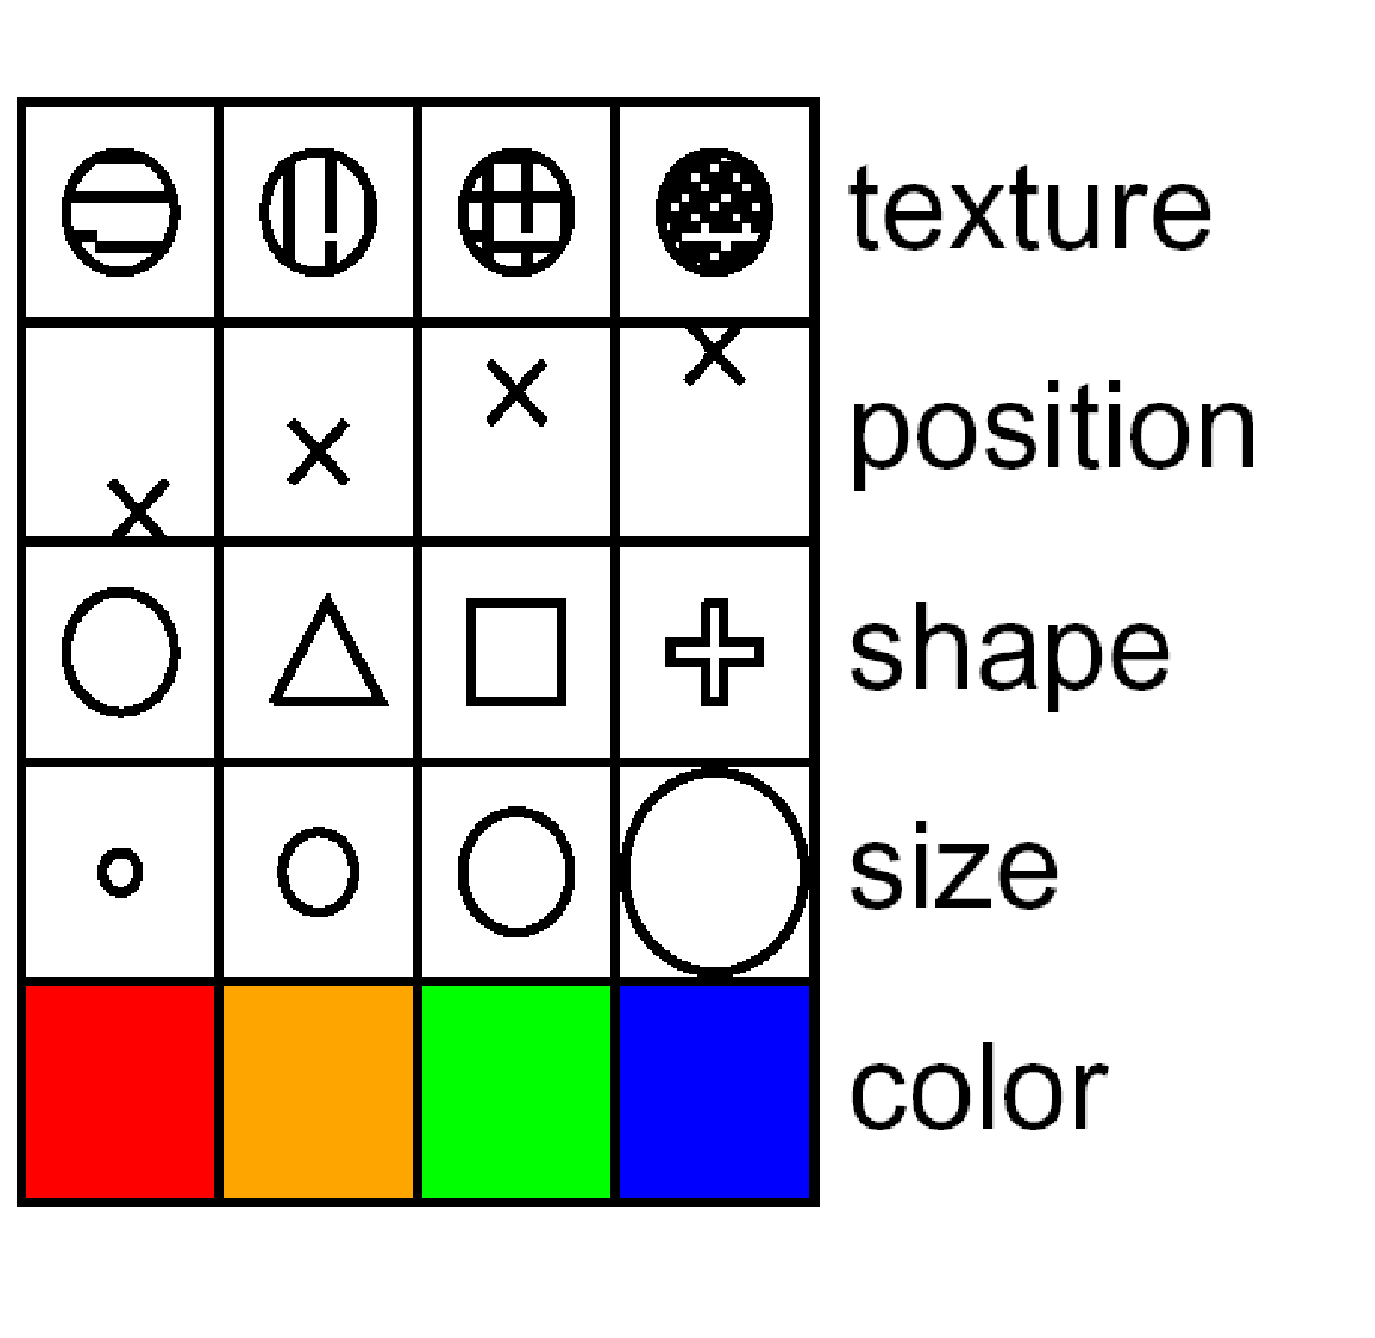
\includegraphics[width=42mm, height=35mm]{figures/xt_stim_layer2.eps}
%\end{center}
%\caption{Stimulus Input Layer: Caricature of input to the XT model, with rows portraying stimulus dimension (color, shape, size, etc) and columns indexing feature values across dimensions (small, medium, large, etc.)}
%\label{stimuluslayer-figure}
%\end{figure} 

The architecture of the XT model is shown in Figure~\ref{xt-layout-figure}. This model makes use of the Leabra framework~\cite{OReillyRC:2000:Computational}. The input of XT consists of two layers of neural units used for the presentation of up to two stimulus objects. It is natural to think of the rows of each input layer as representing different dimensions (e.g., color, shape, texture) and the columns indexing features across each dimension (e.g., red, orange, green, blue). The Response layer has essentially the same structure as an input layer, but includes one additional unit, which codes for ``no response''.  

\begin{figure}
\begin{center}
	\includegraphics[width=125mm]{figures/xt_arch_2.ps}
\end{center}
\caption{XT Model Architecture. The upper left corner shows a
         caricature of the input to the XT network, with rows
         portraying stimulus dimension (color, shape, size, etc.) and
         columns indexing feature values across dimensions (small,
         medium, large, etc.). The AG unit implements ``adaptive gating'' 
	 by modeling the effects of DA on PFC. Adapted from Rougier,
         et al. (2005).}
\label{xt-layout-figure}
\end{figure} 

A collection of Hidden layers map from stimuli to responses. Activity in these layers can be modulated through top-down biasing signals from an actively maintained representation in the PFC layer. Unlike previous models, the actively maintained representations in PFC are learned through a developmental process that involves training the model to perform a variety of simple tasks. These tasks share a need to selectively attend to individual dimensions of the stimuli. The standard synaptic plasticity mechanisms of the Leabra framework, applied over the course of developmental training, produces PFC representations that support focusing attention on a single stimulus dimension at any one time~\cite{RougierNP:2005:XT}.

The Task input indicates which task is to be performed, with one input unit coding for each task. The Dimension Cue layer is used to indicate the currently relevant stimulus dimension, with each unit in the layer corresponding to a specific dimension. All of the Dimension Cue units are turned off for tasks in which the model must discover the relevant dimension on its own.

The flexible adjustment of cognitive control is implemented using a DA-based adaptive gating (AG) mechanism. The model receives a positive scalar reward signal whenever it produces a correct response, and the AG calculates the change in expected future reward: the TD Error. Importantly, the AG, modeling phasic DA responses, not only modulates the learning of reward expectation but also manipulates the ``gate'' on PFC. When the model performs better than expected, the current PFC representation is strengthened. When the model performs worse than expected the current PFC representation is destabilized, allowing a new, possibly more appropriate PFC representation to be entertained~\cite{RougierNP:2005:XT}.

%In the model, the \begin{math}\delta(t)\end{math} value directly modulates excitatory ionic maintenance currents (\begin{math}g_m\end{math} below).  Large maintenance currents drive the membrane potential of simulated neurons in the PFC up, pushing them towards their maximal firing rate.  These currents are not allowed to become negative, being clipped at zero instead.  The maintenance currents, $g_m$, of simulated neurons in PFC are computed by:

%\begin{equation}g_m(t-1) = 0 ~if~ |\delta(t)| > \theta\end{equation}
%\begin{equation}g_m(t)_j = g_m(t-1) + \delta(t) a_j\end{equation}
%\begin{center}$where~a_j~is~the~current~activation~value~of~PFC~unit~j$\end{center}

%Therefore, a positive \begin{math}\delta(t)\end{math} will result in an increase in active maintenance of PFC representations, while a negative \begin{math}\delta(t)\end{math} will destabilize PFC.  The value \begin{math}\theta\end{math} represents a threshold value for the ionic currents.  If the TD error, \begin{math}\delta(t)\end{math}, exceeds this amount (\begin{math}\theta = .5\end{math} in all simulations), then the maintenance currents, \begin{math}g_m\end{math}, are effectively reset.  Over time, the network learns to maintain PFC representations that are likely to result in reward.  


%XT is the first computational cognitive neuroscience model to explore
%the development of PFC representations, and it is the first to provide
%good quantitative fits to both Stroop and WCST data, for both
%neurologically intact and frontally damaged people, based on a biologically informed architecture.

%\subsection{Modeling Autism Using XT}

\subsection{Modeling Autism Using XT}

% \subsubsection{General Approach}

Our theory suggests that a deficit in DA functioning can account for the impaired cognitive flexibility seen in people with autism, while leaving cognitive control robust and relatively unaffected. We have tested this theory by reducing the effect of the DA signal in the XT model by scaling the TD Error (AG) by a constant factor, $\kappa$. The model of typically developing individuals uses $\kappa = 1$, and autism is modeled using $\kappa < 1$. This scaling of the TD Error by $\kappa$ is the only modification from the original XT model that we made. A $\kappa$ value of $0.54$ was found to produce the best fit to human performance. This reduction of the DA signal decreases the efficacy of the PFC gating system, resulting in less efficient destabilization of PFC when errors are made.
%The scaling was only used to modulate the simulated maintenance currents within the PFC layer, and not used to modify the learning of the weights into the Adaptive Gating unit.  An important point of future work is to also test the effects of this manipulation on these weights, weakening the overall influence that dopamine has on learning within circuits involved in the computation of future expected reward, as well.  

%It is worth noting that the modeled DA signal remains agnostic as to the precise quantitative nature of actual DA levels.  It is possible, for instance, that a optimal firing rate of the midbrain DA neurons exists for efficient PFC gating.  This implies \emph{either} too much or too little DA could have deleterious results on the effectiveness (a lower $\kappa$ value) of the DA based PFC gating system.

\subsection{Modeling WCST} 

%The WCST consists of a deck of cards, which contain stimuli varying along three dimensions (e.g., color, shape, quantity) and across four different features per dimension (e.g., for color dimension: red, orange, green, \& blue).  Participants are told to sort the cards into piles, but they are not given any instructions concerning how to do this correctly.  Instead, only sparse feedback ---``Correct'' or ``Incorrect''--- is given upon the placement of each card, until the proper sorting strategy is discovered.  After the sorting rule (e.g., sort by color) is learned by the participant, and $10$ consecutive correct sorts are accomplished, the rule is changed without informing the subject.  This procedure repeats until either $6$ correct categories (sets of $10$ correct consecutive sorts) are achieved, or all $127$ cards in the deck are exhausted.  Errors are recorded as incorrect sorts, with perseverative errors scored as an incorrect sort that used the last correct sorting rule.  Success at WCST requires the ability to flexibly change the dimension being maintained by PFC as the sorting rules change.  Modeling WCST in the XT framework required use of only three of the five possible input dimensions.  The same methods for administrating WCST to human participants were used in these simulations.

\begin{figure}
  \begin{center}
  \resizebox{8cm}{!}{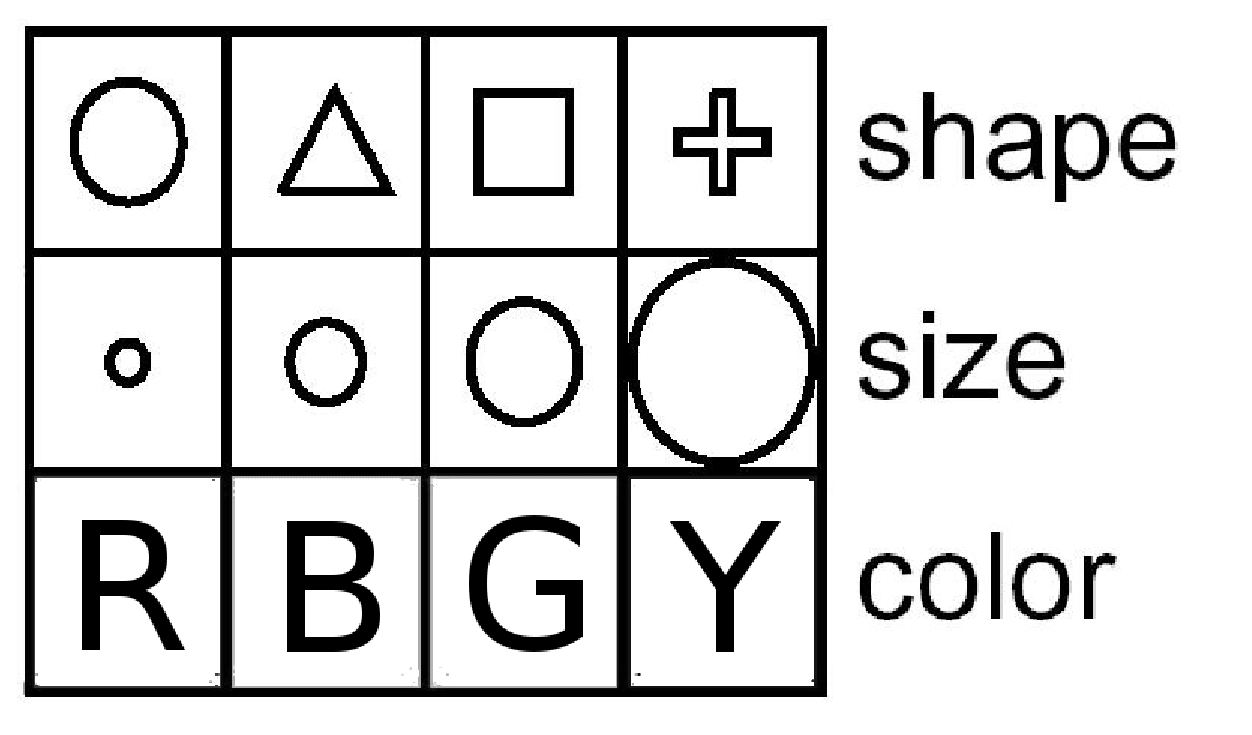
\includegraphics{figures/xt_wcst_stim}}
  \end{center}
  \caption{XT WCST Stimulus Input}
  \label{xt_wcst_stim}
\end{figure}

As in the original XT work, each trial of the WCST was modeled by presenting a single stimulus object ``card'' at the model's inputs, with one unit activated for each feature of the stimulus across three stimulus dimensions. (See Figure~\ref{xt_wcst_stim}.) The model ``sorted'' the ``card'' by outputing the feature of the current stimulus relevant for sorting. For example, when cards were to be sorted by color, the model was expected to output the color of the stimulus (e.g., ``red''). Importantly, the model was not instructed concerning the sorting rule (i.e., the Dimension Cue inputs were all off). Thus, the model needed to search for the relevant stimulus dimension. The model received a positive scalar ``reward'' signal when its output was correct. The use of TD learning to produce AG activity, along with the top-down modulation from PFC, allowed XT to successful learn to focus on the relevant stimulus dimension. The AG mechanism strengthened the maintenance currents of modeled PFC pyramidal cells during good performance, causing the active maintenance of the sorting rule in PFC. When the sorting rule was switched, the actively maintained PFC representation became invalid. Continued active maintenance of PFC firing rates would result in perseverative errors. In the standard XT model, the AG alleviated this problem by providing a gating signal to PFC when reward was expected but not delivered, allowing PFC contents to change~\cite{RougierNP:2005:XT}.

%Four main measures were used in evaluating the performance on the WCST task:

%	1. Total Number of Errors
%
%	2. Percentage of Total Errors 
%
%	3. Total Number of Perseverative Errors
%
%	4. Percentage of Perseverative Errors

%In the XT framework, the Dimension Cue layer is used to inform the network what dimension is currently relevant.  By *not* using this cue, the network is left to figure out what the sorting rule is by feedback alone, analogous to participants in WCST.  Only three of five possible dimensions where used in the stimulus layer in order to facilitate a tighter link with the model to that of the actual WCST task.  

\subsection{Modeling Stroop} 

%Stroop tests cognitive control by measuring the ability to inhibit a prepotent response.  In Stroop, the stimuli are different words presented in various colored fonts.  Participants are asked to either read the word or to name the color of the font in which the text is presented.  People are faster overall at reading the word as opposed to naming the color of the word.  Furthermore, when comparing the neutral (e.g., the word ``house'' in red font) versus the incongruent (e.g., the word ``green'' written in red font) conditions, people are slower in the incongruent case for color naming, but not for word reading.  This is known as Stroop interference.

%Cohen and Servan-Schreiber~(1990)\nocite{CohenJD:1990:Stroop} provided a computational account of the Stroop task. This model incorporated multiple associative pathways from stimulus features to possible responses.  They used a stronger, more automatic word reading pathway through posterior cortex and a relatively weak color naming pathway.  In their model, a task representation, maintained in PFC, provided top-down biasing, injecting extra activity into the color naming pathway when doing so was necessary to overcome the prepotent word reading pathway (i.e., when asked to name the font color).  The resulting competition between the two strong pathways resulted in an increase in response time in the color naming incongruent condition.  Response time was not increased in the word reading incongruent condition, however, as the weaker color naming pathway, when unsupported by PFC, offered little competition.

The XT model performed the Stroop task in much the same way as Cohen's and Servan-Schreiber's seminal model~\cite{CohenJD:1990:Stroop}, leveraging competition between pathways of varying strength: the strong word reading pathway and the weak color naming pathway. In order to simulate this competetion, the frequency of trials in which one dimension (font color) was experienced during development was manipulated. The font color dimension was relevant only 25\% as often as the other dimension, word reading. The time needed for output activity to stabilize was taken as a response time measure~\cite{RougierNP:2005:XT}.
%The settling time, in ``cycles'', of the network was linearly scaled to ``milliseconds'' using a single free parameter, allowing a direct comparison between model results and human data.

\subsection{Simulation Results}

\subsubsection{Simulations} 
Due to stochasticity in model initial conditions and in the sequence of developmental trials, $100$ distinct network models were prepared using the XT training procedure, stopping when a performance criterion was reached, up to a maximum of $100$ training epochs.  Each network was tested under both conditions of DA modulation ($\kappa = 1$ for healthy networks and $\kappa = .54$ for networks modeling ASD), on both WCST and Stroop. Each of the $100$ networks was treated as an individual subject for the purposes of data analysis.

\subsubsection{WCST Results} 
WCST results matched data reported in the literature. The differences between simulated performance of normally functioning individuals and simulated autistic performance were statistically reliable ($p < 0.001$) and consistent with previous studies~\cite{PriorMR:1990:AutismWCST,Ozonoff:1999:AutismStroopWCST,MinshewNJ:2002:AutismWCST}. Specifically, perseverative errors, marking a failure to flexibly discard the initial sorting rule when it was no longer rewarded, were significantly more numerous in the reduced DA modulation version of XT. (See Figure~\ref{ed-results-figure}.)

\begin{figure}
\begin{center}
	\includegraphics[width=110mm]{graphs/wcst.ps}
                                                                
\textcolor{white}{\\--------------------------------\\}

	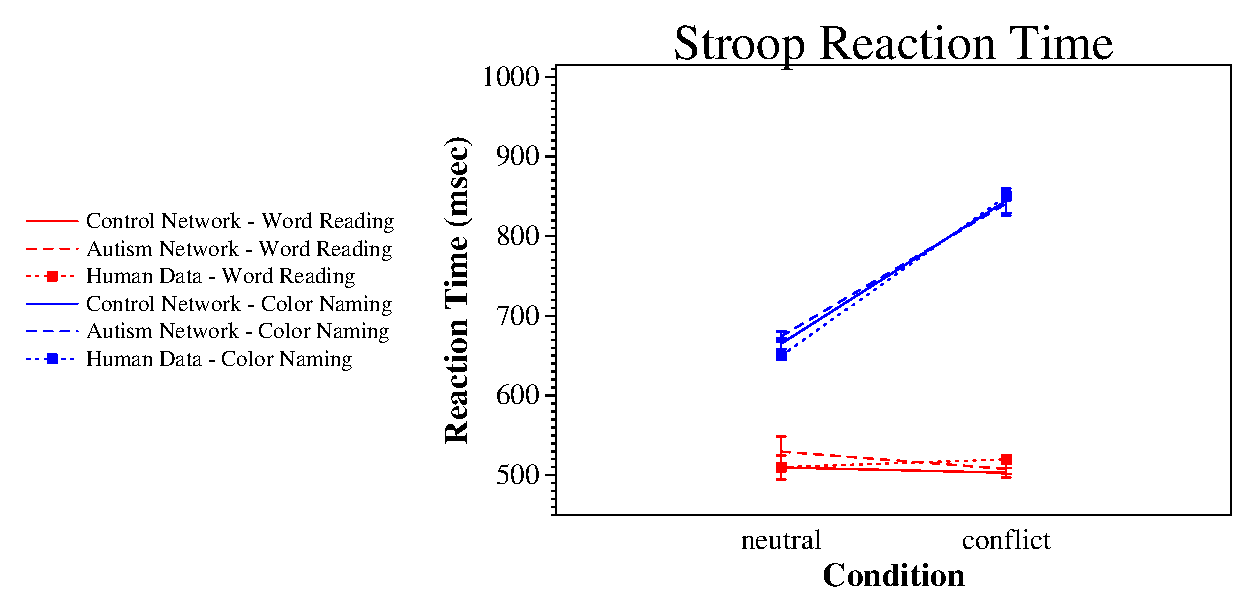
\includegraphics[width=110mm]{graphs/stroop.ps}
\end{center}
\caption{Top: Comparing performance on WCST perseveratitive errors for typically developing and autistic individuals (human data from Minshew, et al., 2002). Error bars are standard errors of the mean. Bottom: Stroop reaction time, comparing simulated performance to human data (healthy human data from~Dunbar, et al.~(1984), and autistic subjects perform no differently than controls~(Ozonoff et al., 1999)).} 
\label{ed-results-figure}
\end{figure} 

\subsubsection{Stroop Results} 
Model performance on the Stroop task provided a good quantitative fit to human performance. (See Figure~\ref{ed-results-figure}.) The model with intact DA function displayed the classic Stroop reaction time results --- slowing for conflict stimuli when color naming. The performance of the ASD model showed no significant increase in Stroop interference in comparison to the healthy model~($F(1,198) = 0.62$; $p > 0.43$), which is consistent with past findings~\cite{Ozonoff:1999:AutismStroopWCST}.

\subsubsection{Developmental Results}
These simulations involved the introduction of a DA deficit only after the model was fully developed. Thus, these simulations ignored the possibility that an early manifestation of a DA deficit might hinder the proper learning of PFC representations, introducing an impairment in cognitive control in the model that is not observed in autistic subjects. To address this issue, the DA deficit in the ASD model was introduced prior to developmental training. PFC development and model performance were analyzed over the entire developmental period of the model ($100$ epochs). Two groups of $10$ networks were used: an autistic group with $\kappa = 0.54$ and a control group with $\kappa = 1.00$. At the end of developmental training, the networks exhibited the same pattern of results as seen in the initial simulations. Furthermore, we found that the DA deficit did not hinder the learning of useful PFC representations, allowing for focused attention on a single stimulus dimension.

% Furthermore, careful examination of the development of the PFC representations provided some insight into why executive deficits might appear late in autism, as described in the literature~\cite{GriffithEM:1999:AutismYoungED}.  

% \subsubsection{PFC Representations} 

% Figures~\ref{rep1-figure} and \ref{rep2-figure} plot the synaptic strengths from the PFC layer to the Response layer.  Each large box corresponds to a PFC unit, and each encapsulated small box corresponds to a Response unit, with the strength of the connection from the given PFC unit to the given Response unit being reflected in the brightness of the box (lighter means stronger).  Note that each row designates connections to Response layer units representing features in the same stimulus dimension.  (See the upper left corner of Figure~\ref{xt-layout-figure}.)  Thus, these plots can be used to examine the degree to which the PFC layer developed a representational scheme that allowed for the selective modulation of individual stimulus dimensions.  For a given PFC unit (large box), a bright row of connections (small boxes) indicates that that unit selectively supports attention to the stimulus dimension corresponding to that row.  In Figure~\ref{rep1-figure}, which was generated early in developmental training, both the autistic network and the control network lack strong dimensional weights.  However, in Figure~\ref{rep2-figure}, both networks have developed strong dimensional representations in PFC, as evidenced by the extremely salient horizontal bands of ``strong'' weights.  Thus, appropriate PFC representations were acquired only slowly over the course of developmental training, and the DA manipulation did not hinder the formation of these representations.

% \begin{figure}[t]
% \begin{center}
% 	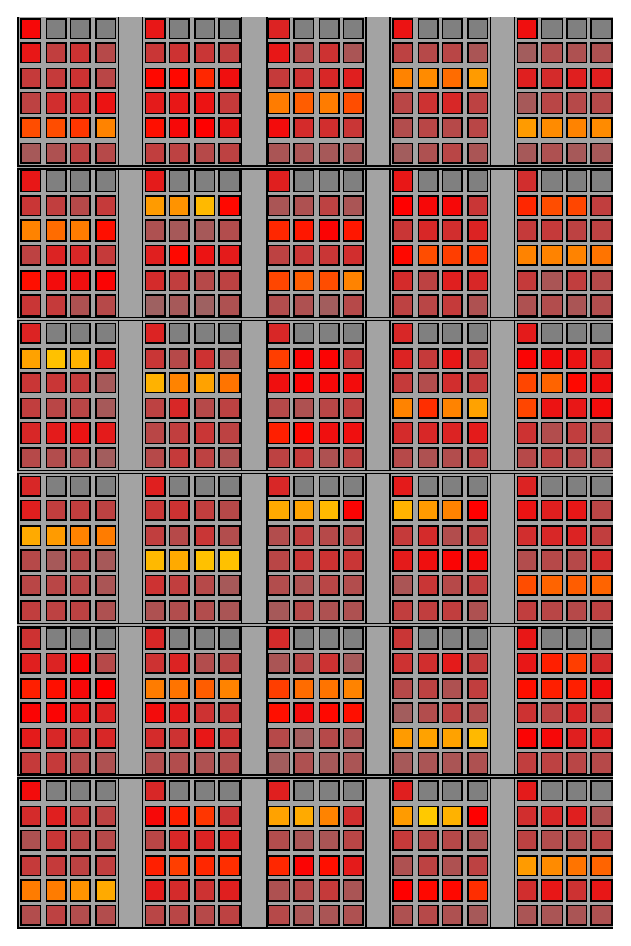
\includegraphics[width=35mm,height=55mm]{graphs/PFCwts1.05.eps}
% 	\hspace{18 mm}
% 	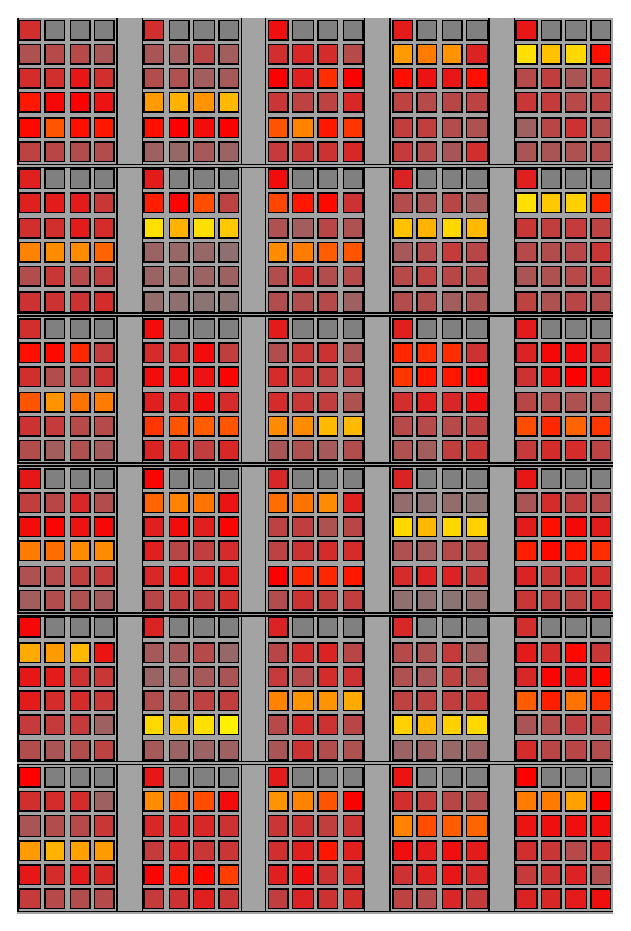
\includegraphics[width=35mm,height=55mm]{graphs/PFCwts54.05.eps}
% \end{center}
% \caption{PFC Representations early in development
%          (epoch 5): left - control model, right -
%          autism model.}
% \label{rep1-figure}
% \end{figure} 

% \begin{figure}[th]
% \begin{center}
% 	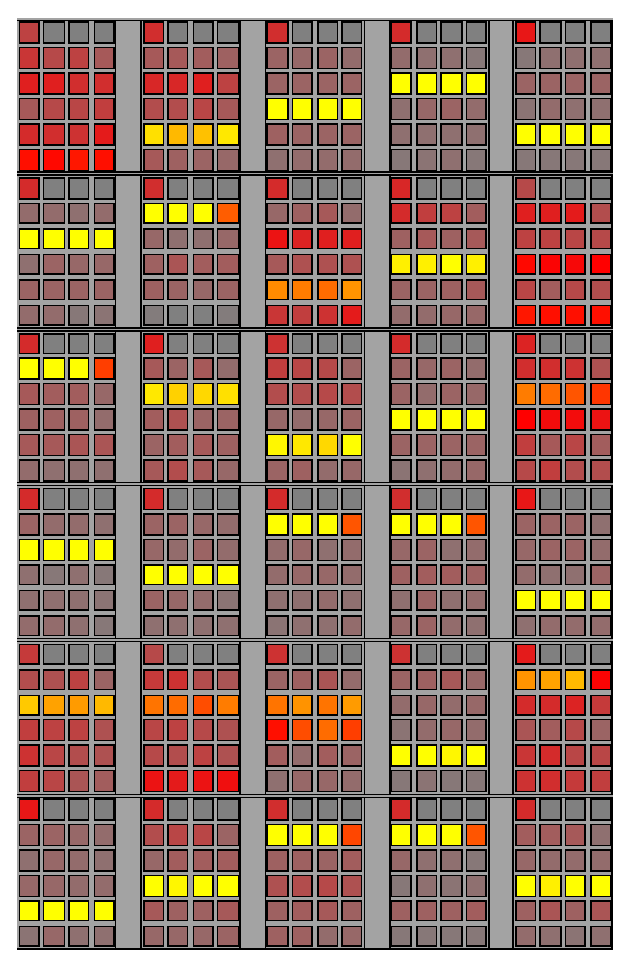
\includegraphics[width=35mm,height=55mm]{graphs/PFCwts1.100.eps}
% 	\hspace{18 mm}
% 	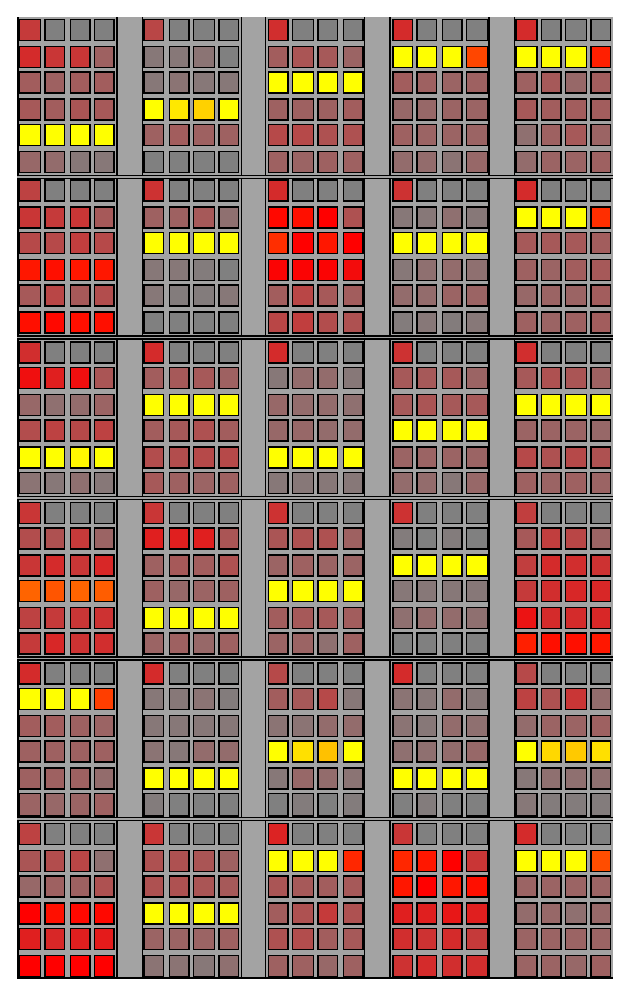
\includegraphics[width=35mm,height=55mm]{graphs/PFCwts54.100.eps}
% \end{center}
% \caption{PFC Representations late in development
%          (epoch 100): left - control model, right -
%          autism model.}  
% \label{rep2-figure}
% \end{figure} 

% \subsubsection{Executive Dysfunction Development} 

Interestingly, these simulations offer a potential explanation for the observation that cognitive flexibility deficits, in comparison to controls, appear late in development~\cite{GriffithEM:1999:AutismYoungED}. In Figures~\ref{stroop-devel-figure}~\&~\ref{wcst-devel-figure}, the Stroop interference effect and the number of perseverative errors in WCST are plotted over developmental training time. Figure~\ref{stroop-devel-figure} shows no effect of the DA manipulation across development. Stroop interference was significantly greater for the autistic networks during only $1$ training epoch out of the $100$ ($p < 0.003$), demonstrating robust cognitive control throughout development. Figure~\ref{wcst-devel-figure}, however, shows a significant difference in perseverative errors only after an initial period of developmental training. During the first $53$ epochs there was a significant difference ($p < 0.05$) during only $26.4\%$ of the epochs, but later in development (epochs $54-100$) a significant difference was reached $93.6\%$ of the time. Importantly, neither healthy nor autistic models showed a distinct advantage or disadvantage during the earliest stages of development. We conjecture that early poor performance by both model types was largely due to the fact that strong, dimensionally selective, PFC representations had yet to learned. Without such PFC representations, the networks were forced to rely more heavily on synaptic plasticity in the Hidden layers (posterior cortex) to perform the tasks. Later in development, both healthy and autistic networks acquired good PFC representations, but the models with reduced DA influence on PFC displayed difficulties in updating those representations when expected reward stopped being delivered (i.e., when the sorting rule was changed).

\subsection{Summary}

These simulations show that, given the XT account of the role of PFC in executive control, reducing the influence of DA on PFC adaptive gating is sufficient to capture the pattern of performance exhibited by people with autism on tests of cognitive flexibility (WCST) and cognitive control (Stroop). Furthermore, we demonstrated that weakening the DA signal over the course of PFC development continues to reflect autistic performance, while also providing some insight into the late appearance of cognitive flexibility deficits in autism. More information about these simulations may be found in Kriete \& Noelle~(2015).\nocite{KrieteT:2015:ED}

\begin{figure}[t]
\begin{center}
	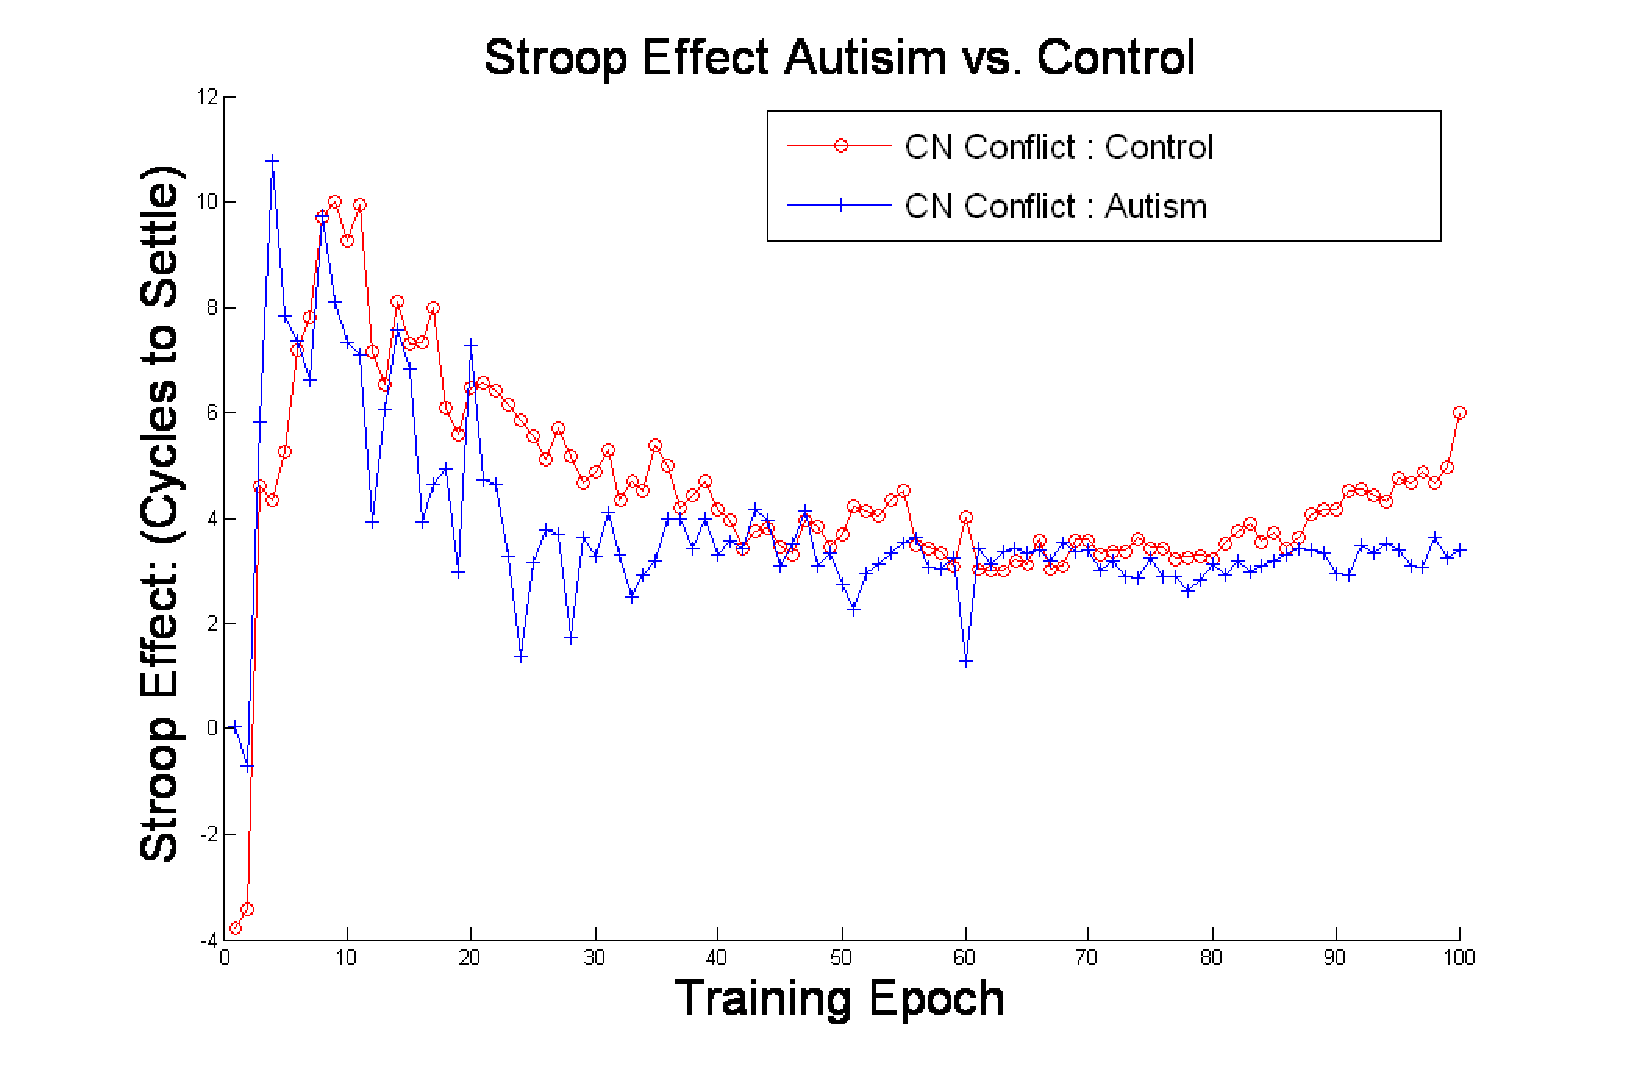
\includegraphics[width=145mm]{graphs/stroop_devel.eps}
\end{center}
\caption{Model Stroop Interference Over the Course of Development.} 
\label{stroop-devel-figure}
\end{figure} 

\begin{figure}[t]
\begin{center}
	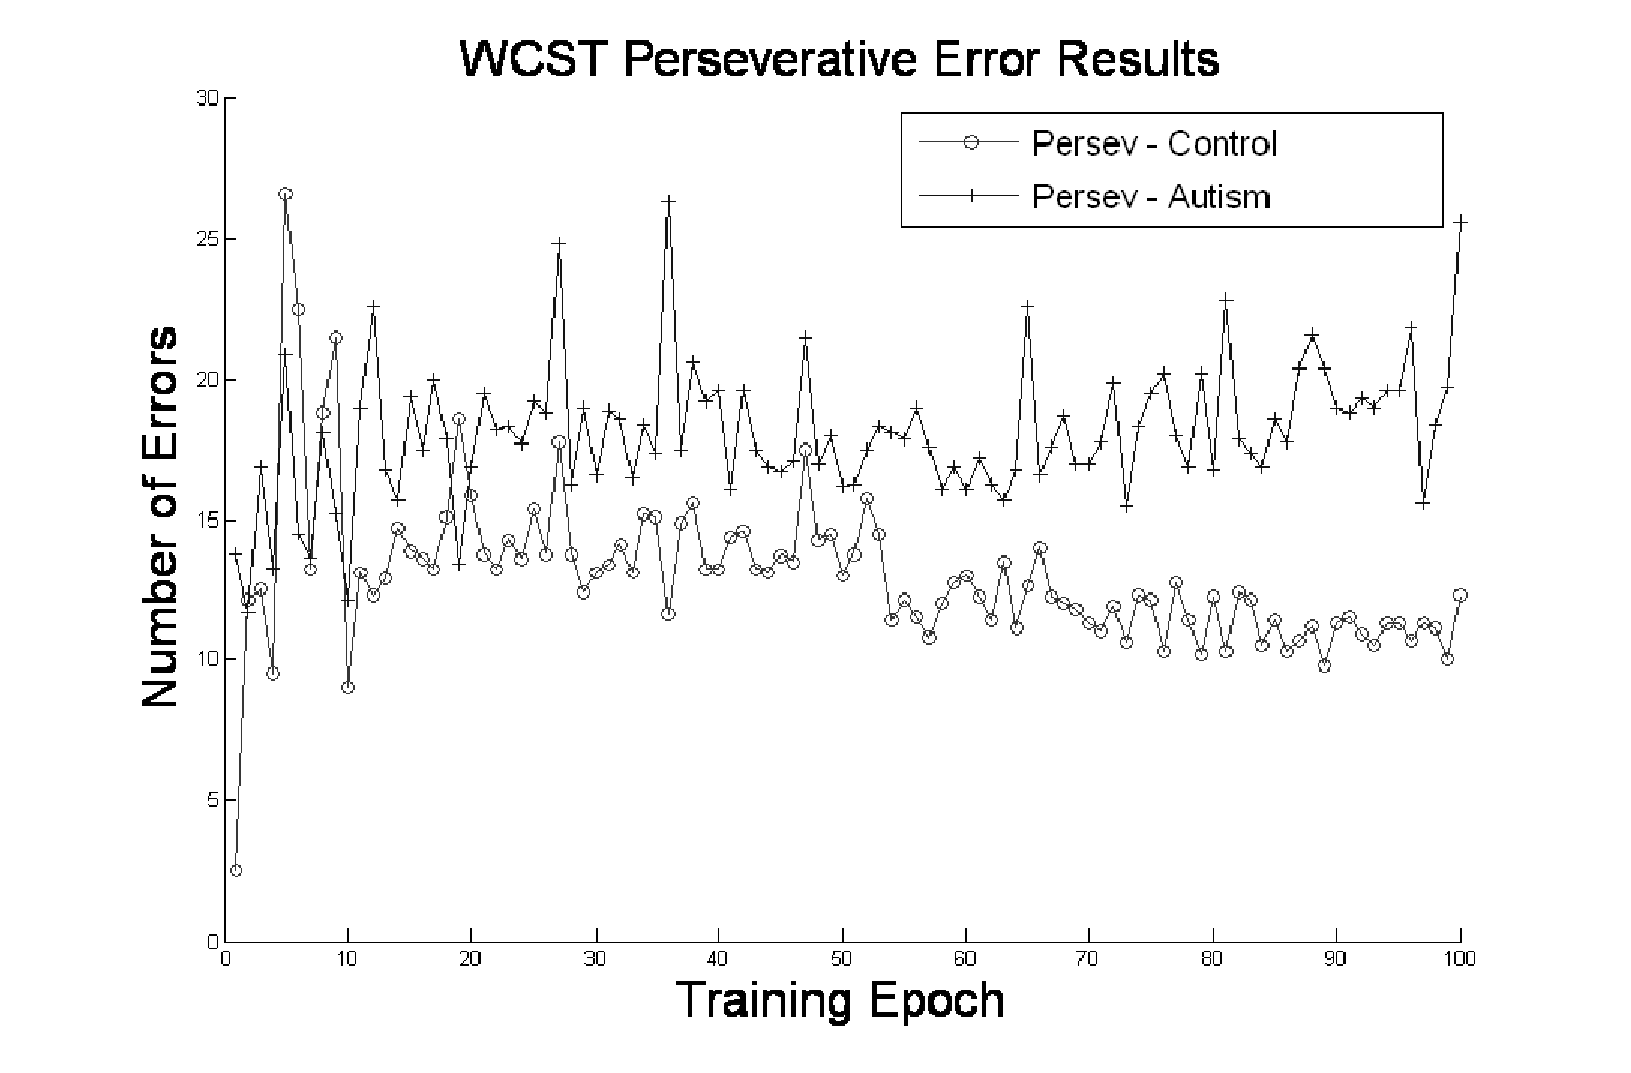
\includegraphics[width=145mm]{graphs/wcst_devel_persev.eps}
\end{center}
\caption{Model WCST Perseverative Error Count Over the Course of Development.} 
\label{wcst-devel-figure}
\end{figure} 

